\section{Experimental setup} \label{experimental_setup}

\subsection{Data preparation}

To prepare a central dataset, both single datasets had to be transformed into a common format. For the central dataset only the class and the text content of each tweet respectively each forum contribution was considered.

The first dataset \citetitle{ThomasDavidson2020} was entirely given as a .csv file and contains around 25k tweets, that were either labeled as hate speech, offensive language or neither of both. To determine the right label three independent evaluators classified each tweet, the final label got assigned by the majority vote. As for the first approach, one is only interested in hate speech and neutral tweet classification, all offensive language documents in the dataset were dropped. Some tweets were retweets that were commented additionally by a user. An example is shown below:

\begin{quote}
    """@DevilGrimz: @VigxRArts you're fucking gay, blacklisted hoe"" Holding out for \#TehGodClan anyway http://t.co/xUCcwoetmn"
\end{quote}

The original tweets can be found in between the ""..."". As it could not be distinguished whether the original tweet or the retweet contains hate speech, these documents were filtered out in the first version of the preprocessing pipeline. Same goes for tweets that cite other users without using the retweet option. Once the semantic feature for the number of quotes was added, the removal of quoting tweets was reverted again. Probably it is still expected behavior in social media platforms to remove contributions that build up on hate speech. 

The second dataset \citetitle{DeGibert2020} was not entirely given as a .csv file. Only the document annotations were given in a .csv file, all forum contributions were stored in separate .txt files. Only documents which could not be assigned to a single class (label "idk/skip") or referred to other documents (label "relation") were dropped.

The resulting common dataset was stored in a .csv file. It contains 2.626 hate speech documents and 13.670 non hate speech documents. The dropped offensive language documents make up 19.196 instances. 

\subsection{Corpus building}

The common dataset is loaded from the .csv file into a pandas dataframe. After doing basic preprocessing like lowercasing and removing emojis and other irrelevant characters, spacy is used to build a tokenized corpus. The language model from spacy decides about stop word, punctuation and white space removal. No hard coded logic or stop word lists are used in this process. This keeps URLs or other tokens including punctuation as one token. 

Regarding tokenization using the lemmas instead of word stems works better as for instance \textit{we'll} becomes \textit{["we","will"]} and not \textit{["we", "'ll"]}. For getting n-gram features, the lemmatized tokens are stemmed. This keeps the range of possible unigrams for one and the same semantic word instance restricted. PoS tags are added to the dataframe using NLTKs PoS tagger as problems using spacys PoS tagger were encountered. PoS-tags are necessary for the hate speech pattern extraction.

Depending on the method the inputs vary. For the conventional machine learning methods the inputs are the extracted features as numerical values added to the dataframe by the already mentioned \textit{Feature\-Extractor} class, whereas in neural network based approaches the inputs are the raw textual contents of each document and the embeddings are learned automatically. The labels are in both cases numerical values.

Then we perform the dataset balancing. As already mentioned, the acquired dataset is an imbalanced one, which can lead to a decrease in performance and accuracy with machine learning classification. As a comparison Oriola and Kotz\'{e} \cite{Oriola.2020} recognized the class imbalance and tried to reduce it by applying a synthetic minority oversampling technique called SMOTE \cite{Chawla2011}. In general there are a few possibilities to tackle the challenge of unbalanced classes:

\begin{itemize}
    \item changing the performance metric (e.g. F1-score instead of accuracy)
    \item undersampling, i.e. deleting instances from the over-represented class
    \item oversampling, i.e. adding copies of instances from the under-represented class
    \item generating synthetic samples (e.g by using SMOTE)
\end{itemize}

In our experiments we chose to try the different approaches and applied a simple undersampling by randomly deleting instances from the over-represented class (neutral posts), as well as an oversampling using SMOTE. SMOTE does an oversampling by generating synthetic samples in the feature-space of the under-represented class, resulting in posts that statistically fall in between the different hate speech posts. Additionally, we used the imbalanced dataset to train a classifier to compare how this affects the performance.
Finally we receive unbalanced, undersampled and oversampled datasets, which we use for the further experiments. In addition for all experiments, we use the F1-score instead of the accuracy as our performance metric, which should somewhat handle unbalanced classes by itself.

Unfortunately, SMOTE only works in feature space, so we could not provide an oversampled balanced dataset for our neural network approach as this works directly on the hate speech and non-hate speech posts. This could be addressed in future work.

\subsection{Data insights} \label{sec:data_insights}

To better understand the dataset we are working with, the following section provides some insights into the preprocessed data corpus.
In an in-depth analysis of the data, we had a look at the length of hate speech posts versus non-hate speech posts. This can be seen in \autoref{fig:post_length_density_distribution}.

\begin{figure}[ht]
    \centering
    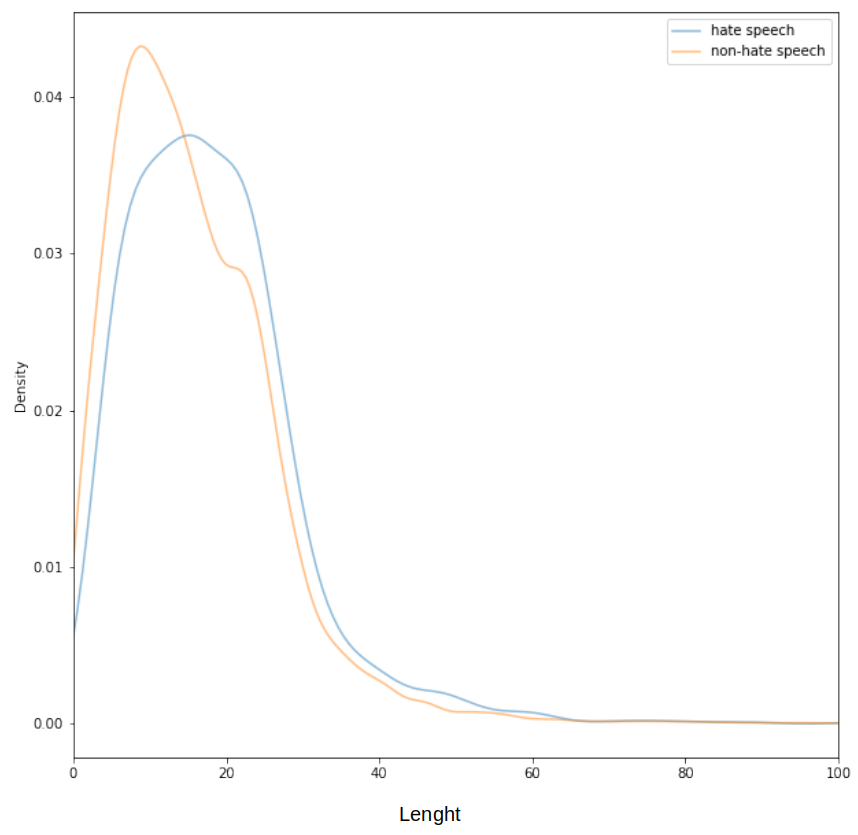
\includegraphics[width=0.8\linewidth]{figures/post_length_density_distribution.png}
    \caption{Density distribution of the length of a post (tweet or forum post)}
    \label{fig:post_length_density_distribution}
\end{figure}

Here one can see, that the hate speech posts contain more words (tokens before cleaning) than non-hate speech posts. In average a hate speech post contains 18.18 words, whereas a non-hate speech post only contains 15.85 words. Unlike expected, the hate speech posts are longer than the non-hate speech posts.

A more interesting look at the data is given by the most commonly used words per class. As can be seen in the word clouds in \autoref{fig:wordclouds} there are some obvious differences. The hate speech posts use words like \enquote{bitch}, \enquote{faggot} or \enquote{nigga}. But interestingly enough, the non-hate speech posts also sometimes consist of the words \enquote{trash} or \enquote{white}.

\begin{figure}[ht]
    \hfill
    \begin{subfigure}[b]{0.4\textwidth}
        \centering
        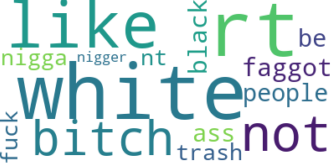
\includegraphics[width=\textwidth]{figures/Wordcloud-HateSpeech-tokens.png}
        \caption{hate speech}
    \end{subfigure}
    \hfill
    \begin{subfigure}[b]{0.4\textwidth}
        \centering
        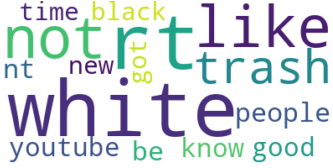
\includegraphics[width=\textwidth]{figures/Wordcloud-Non-HateSpeech-tokens.png}
        \caption{non-hate speech}
    \end{subfigure}
    \hfill
    \caption{Word clouds}
    \label{fig:wordclouds}
\end{figure}

For a better insight into our data, a few examples are shown in the following.

\noindent
Examples for non-hate speech (neutral sentences):
\begin{itemize}
    \item "billy that guy wouldn't leave me alone so i gave him the trudeau salute"
    \item "this is after a famous incident of former prime minister pierre trudeau who gave the finger to a group of protesters who were yelling antifrench sayings at him"
    \item "askdems aren't you embarrassed that charlie rangel remains in your caucus"
\end{itemize}

\noindent
Examples for hate speech:
\begin{itemize}
    \item "california is full of white trash"
    \item "and yes they will steal anything from whites because they think whites owe them something so it's ok to steal"
    \item "why white people used to say that sex was a sin used to be a mystery to me until i saw the children of browns and mixed race children popping up all around me"
\end{itemize}

One can clearly see the hate expressed in the hate speech examples and see their discriminating nature.

\subsection{Experimental details}

The optimal hyperparameters of the conventional machine learning methods are learned automatically as part of the pipeline. Nevertheless the learned optimal hyperparameters are listed in the appendix \ref{ch:app-A} to enable the replication of our results. For readability only the hyperparameters differing from the default values are listed.
